\documentclass{article}

%table customization, stack overflow 
\usepackage{array}
\newcolumntype{L}[1]{>{\raggedright\let\newline\\
\arraybackslash\hspace{0pt}}m{#1}}

%figure flaots from http://www.tex.ac.uk/FAQ-figurehere.HTML
\usepackage{float}

\usepackage{tabularx}
\usepackage{enumitem}
\usepackage{graphicx}
\usepackage{booktabs}
\usepackage{url}
\usepackage{hyperref}
\usepackage{fancyhdr}
\pagestyle{fancy}
\begin{document}
\pagenumbering{gobble}
\lhead{Team 6\\ JSTanks\\}
\newpage
\title{JSTanks - Test Plan}
\date{December 8, 2016}
\author{Jiahao Li\\LI577\\001416646\and Pavithran Pathmarajah\\PATHMAP\\
001410729 \and Viren Patel\\PATELVH3\\001419057}

\maketitle

\newpage
\pagenumbering{arabic}
\tableofcontents
\newpage
\listoftables

\newpage
\listoffigures

\newpage
\section{Revision History}
\subsection{Revision 0}
\begin{table}[H]
\caption{Revision 1}
	\begin{tabularx}{\textwidth}{cXc}
		\toprule
		Date & Developer & Change\\
		\midrule
		October 31&Jiahao Li &Initial Draft \\
		October 31&Pavithran Pathmarajah &Initial Draft\\
		October 31&Viren Patel  &Initial Draft\\
	\end{tabularx}
\end{table}

\subsection{Revision 1}
\begin{table}[H]
\caption{Revision 2}
	\begin{tabularx}{\textwidth}{cXc}
		\toprule
		Date & Developer & Change\\
		\midrule
		December 6&Pavithran Pathmarajah & Update Tests Performed\\
		October 31&Viren Patel  &Spelling and Grammer\\
	\end{tabularx}
\end{table}



\section{General Information}
\subsection{Purpose}
This document is a plan for the testing, validation and verification process 
that are to be followed by JSTanks after the build process. These test cases 
were designed prior to the development of the final product; this test plan 
should be used as guidelines and for reference in the final product testing. 

\subsection{Scope}
This project is being designed to move from running local applets that require 
compilation to an on-line script interpreted by browsers. Therefore the 
testing will mainly consists of the teams ability to port java coding 
methodologies and object oriented styles, to Javascript. The testing will 
cover, algorithms, data structures, visuals and the system. 

\subsection{Acronyms, Abbreviations, and Symbols}
\begin{figure}[H]
	\centering
	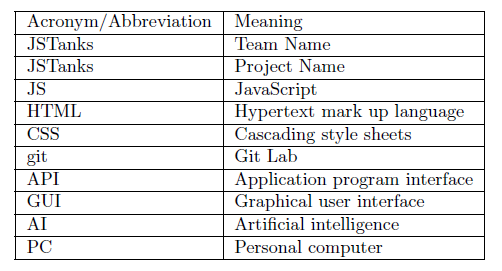
\includegraphics[width=\textwidth]{fig1.png}
	\caption{Acronyms}
\end{figure}

\subsection{Overview of Document}
This document is divided into sections and within each section subsections for 
different test types. There is the general information section covering 
information for the document. The plan for how the product will be tested the 
schedule and the tools used, The system tests to be performed functional and 
non-functional. Followed by the tests for the proof of concept demonstration, 
comparisons to the original Java code. Unit testing to be performed as well as 
the appendix. 

\section{Plan}
\subsection{Software Description}
JSTanks is a game which allows users enjoy it on a website without downloading 
it. This game let the user control a tank to fire and move on the map in order 
to protect its home base and itself from the damage of other tanks'.
\subsection{Test Team}
The test team will consist of Jiahao Li, Pavithran Pathmarajah, Viren Patel 
and some random players as testers. Jiahao Li, Pavithran Pathmarajah, Viren 
Patel will split the entire testing which cover all different types of tests. 
The random player will test the performance of the game and give feedbacks to 
the development team.

\subsection{Automated Testing Approach}
For automated testing we plan to approach the topic through, the use of 
a secondary Script so that we may brute force many scenarios in a short period 
of time, and then be able to debug and run the same set of tests on the 
product again, until all tests are passed and debugging is completed. To save 
time as compared to having to manually enter the same tests each time.

\subsection{Testing Tools}
For testing we plan to use web-browsers and a testing script. We plan to use
Mozilla Firefox, Google Chrome, and Apple Safari browsers to ensure that our
tests pass on the three main browsers used today. We plan to do manual testing
as well as automated testing via a custom made script tailored to our testing
plan.

\subsection{Testing Schedule}
Below is our planned testing schedule broken down into milestones.

%proof of concept
\begin{table}[H]
\caption{Milestone 1 - Proof of Concept}
	\begin{tabularx}{\textwidth}{| c | l | X | l |}
	\toprule
	Test \#& Team Member &Comments &Date\\
	\midrule
	4.1.1 & Pavithran Pathmarajah & All Scripts load up & 10\textbackslash15
	\textbackslash 2016\\
	5.1 & Pavithran Pathmarajah & HTML-5 Canvas functional & 10\textbackslash15
	\textbackslash2016\\
	5.2 & Pavithran Pathmarajah & Keyboard interface functional & 10
	\textbackslash15\textbackslash2016\\
	5.3 & Pavithran Pathmarajah & Update scripts functional & 10\textbackslash
	16\textbackslash2016\\
	\bottomrule
	\end{tabularx}
\end{table}

%gamemenus
\begin{table}[H]
\caption{Milestone 2 - WebPage}
	\begin{tabularx}{\textwidth}{| c | l | X | l |}
	\toprule
	Test \#& Team Member &Comments &Date\\
	\midrule
	4.1.2 & Automated Script   & SUCCESSFUL & 12\textbackslash
	6\textbackslash2016\\
	4.1.3 & Automated Script  & SUCCESSFUL & 12\textbackslash
	6\textbackslash2016\\
	4.1.4 & Automated Script  & SUCCESSFUL & 12\textbackslash
	6\textbackslash2016\\
	4.1.6 & Automated Script  & SUCCESSFUL & 12\textbackslash
	6\textbackslash2016\\
	\bottomrule
	\end{tabularx}
\end{table}

%game & menus
\begin{table}[H]
\caption{Milestone 3- Menus}
	\begin{tabularx}{\textwidth}{| c | l | X | l |}
	\toprule
	Test \#& Team Member &Comments &Date\\
	\midrule
	4.1.5 & Automated Script  & SUCCESSFUL & 12\textbackslash
	6\textbackslash2016\\
	4.1.7 & Automated Script  & SUCCESSFUL & 12\textbackslash
	6\textbackslash2016\\
	4.1.8 & Automated Script  & SUCCESSFUL & 12\textbackslash
	6\textbackslash2016\\
	4.1.9 & Automated Script  & SUCCESSFUL & 12\textbackslash
	6\textbackslash2016\\
	4.1.10 & Automated Script  & SUCCESSFUL & 12\textbackslash
	6\textbackslash2016\\
	4.1.11 & Automated Script  & SUCCESSFUL & 12\textbackslash
	6\textbackslash2016\\
	4.1.15 & Automated Script  & SUCCESSFUL & 12\textbackslash
	6\textbackslash2016\\
	\bottomrule
	\end{tabularx}
\end{table}

%game
\begin{table}[H]
\caption{Milestone 4 - Game}
	\begin{tabularx}{\textwidth}{| c | l | X | l |}
	\toprule
	Test \#& Team Member &Comments &Date\\
	\midrule
	4.1.13 & Automated Script  & SUCCESSFUL & 12\textbackslash
	6\textbackslash2016\\
	4.1.14 & Automated Script  & SUCCESSFUL & 12\textbackslash
	6\textbackslash2016\\
	4.1.16 & Pavithran Pathmarajah
	  & Tank continuously moves in specified directoon & 
	  12\textbackslash
	6\textbackslash2016\\
	4.1.17 & Automated Script  & SUCCESSFUL & 12\textbackslash
	6\textbackslash2016\\
	4.1.18 & Automated Script  & SUCCESSFUL & 12\textbackslash
	6\textbackslash2016\\
	4.1.19 & Automated Script  & SUCCESSFUL & 12\textbackslash
	6\textbackslash2016\\
	4.1.20 & Automated Script  & SUCCESSFUL & 12\textbackslash
	6\textbackslash2016\\
	4.1.21 & Automated Script  & SUCCESSFUL & 12\textbackslash
	6\textbackslash2016\\
	4.1.22 & Automated Script  & SUCCESSFUL & 12\textbackslash
	6\textbackslash2016\\
	4.1.23 & Automated Script  & SUCCESSFUL & 12\textbackslash
	6\textbackslash2016\\
	4.1.24 & Automated Script  & SUCCESSFUL & 12\textbackslash
	6\textbackslash2016\\
	4.1.25 & Automated Script  & SUCCESSFUL & 12\textbackslash
	6\textbackslash2016\\
	4.1.26 & Automated Script  & SUCCESSFUL & 12\textbackslash
	6\textbackslash2016\\
	4.1.27 & Automated Script  & SUCCESSFUL & 12\textbackslash
	6\textbackslash2016\\
	4.1.28 & Automated Script  & SUCCESSFUL & 12\textbackslash
	6\textbackslash2016\\	\bottomrule
	\end{tabularx}
\end{table}

%Unit Tests
\begin{table}[H]
\caption{Unit Tests}
	\begin{tabularx}{\textwidth}{| c | l | X | l |}
	\toprule
	Test \#& Team Member &Comments &Date\\
	\midrule
	7.1.1 & Automated Script  & SUCCESSFUL & 12\textbackslash
	6\textbackslash2016\\
	7.1.2 & Automated Script  & SUCCESSFUL & 12\textbackslash
	6\textbackslash2016\\
	7.1.3 & Automated Script  & SUCCESSFUL & 12\textbackslash
	6\textbackslash2016\\
	7.1.4 & Pavithran Pathmarajah& Wall on screen& 12\textbackslash
	6\textbackslash2016\\
	7.1.5 & Pavithran Pathmarajah& Steel screen & 12\textbackslash
	6\textbackslash2016\\
	7.1.6 & Pavithran Pathmarajah& Base on screen & 12\textbackslash
	6\textbackslash2016\\
	7.1.7 & Automated Script  & SUCCESSFUL & 12\textbackslash
	6\textbackslash2016\\
	7.1.8 & Automated Script  & SUCCESSFUL & 12\textbackslash
	6\textbackslash2016\\
	7.1.9 & Automated Script  & SUCCESSFUL & 12\textbackslash
	6\textbackslash2016\\
	7.1.10 & Automated Script  & SUCCESSFUL & 12\textbackslash
	6\textbackslash2016\\
	7.1.11 & Automated Script  & SUCCESSFUL & 12\textbackslash
	6\textbackslash2016\\
	7.1.12 & Automated Script  & SUCCESSFUL & 12\textbackslash
	6\textbackslash2016\\
	7.1.13 & Automated Script  & SUCCESSFUL & 12\textbackslash
	6\textbackslash2016\\
	7.1.14 & Pavithran Pathmarajah& Visible on screen & 12\textbackslash
	6\textbackslash2016\\
	7.1.15 & Automated Script  & SUCCESSFUL & 12\textbackslash
	6\textbackslash2016\\
	7.1.16 & Automated Script  & SUCCESSFUL & 12\textbackslash
	6\textbackslash2016\\
		\bottomrule
	\end{tabularx}
\end{table}



\section{System Test Description}
\subsection{Tests for Functional Requirements}
\subsubsection{HTML file test}
Name:  Loading the game \newline
Description: Test if the game dependencies load in browser
\newline
Type: Unit test (dynamic, automatic, black box) \newline
Initial State:  Testing Script Loaded in \newline
Input: Click the Run Script button \newline
Output: Script is successful, Loads Dependencies \newline
Pass:  All files are able to be loaded up. \newline

\subsubsection{Standby state test}
Name:  Standby state\newline
Description: Test if the game automatically runs or waits
for user initialization. \newline
Type: Unit test (static, manual, black box) \newline
Initial State: A new browser \newline
Input: Go to home page of game \newline
Output: The home page of the game \newline
Pass: The browser remains on the home page. \newline

\subsubsection{The game section of the menu test}
Name: Menu of game section\newline
Description: Test if the sub menu of new game section which has choices of 
level selection and map selection show up.
\newline
Type: Unit test (dynamic, automatic, black box) \newline
Initial State: Menu in the standby state \newline
Input: Script selects new game \newline
Output:  Menu Tests successfully  \newline
Pass: The sub menu with choice of starting a new game and quit. \newline

\subsubsection{The pause section of the menu test}
Name:  Menu representation\newline
Description: check if the menu contains Home Page/Continue/
Instructions/New Game/Quit \newline
Type: Unit test (dynamic, automatic, black box) \newline
Initial State: A new browser \newline
Input: Click the Run Script button \newline
Output: Menu Tests successfully \newline
Pass: The menu with five sections is represented in the standby state. \newline

\subsubsection{The level section of the menu test}
Name:  Menu of level\newline
Description: Test if the sub menu of level section which has choices of level 
1, level 2, and level 3 shows up when the level section is clicked. \newline
Type: Unit test (dynamic, automatic, black box) \newline
Initial State: Menu in the new game state \newline
Input: Script runs through levels\newline
Output: New Game Success\newline
Pass: The sub menu with choice of level 1, level 2, level 3, level 4 and level 5. \newline

\subsubsection{Game start test}
Name:  Start the game\newline
Description: Test if the game shall be reset and start when [starting a new 
game] is clicked. \newline
Type: Unit test (dynamic, automatic, black box) \newline
Initial State:  The sub menu of the game section \newline
Input: Click the choice of starting a new game \newline
Output: New Game Success\newline
Pass: The standby state of the game with all objects on their initial position 
on the map. \newline

\subsubsection{Game quit test}
Name:  Quit the game\newline
Description: Test if the game comes to ends and the user is redirected to
 the repo if the quit is clicked \newline
Type: Unit test (dynamic, automatic, black box) \newline
Initial State:  The running state of the game \newline
Input: Click the Quit option\newline
Output: Menu Tests successfully \newline
Pass: The game is redirected to the gitlab repository.  \newline

\subsubsection{Game pause test}
Name:  Pause the game\newline
Description: Test if the game comes to the pause state when the letter 'p' is 
pressed on the keybaord. \newline
Type: Unit test (dynamic, automatic, black box) \newline
Initial State: The running state of the game \newline
Input: Script triggers a keyboard event 'p'\newline
Output: The game pauses and the pause menu shows up \newline
Pass: The game comes to a pause state. Game content freezes and 
stays in the temporal positions whilst the Pause menu is overlayed . \newline

\subsubsection{Game continue test 0}
Name:  Continue the game\newline
Description: Test if the game comes back to the running state state when the letter 'p' is 
pressed on the keyboard. \newline
Type: Unit test (dynamic, automatic, black box) \newline
Initial State: The pause state of the game\newline
Input: Script triggers a keyboard event 'p'\newline
Output: The game resumes \newline
Pass: All stuff frozen in the pause state are activated and back into the 
routine. \newline

\subsubsection{Game continue test 1}
Name:  Continue the game in the running state\newline
Description: Test if there is any effect on the game when the choice of 
continue is clicked in the running state. \newline
Type: Unit test (dynamic, automatic, black box) \newline
Initial State: The running state of the game \newline
Input: Script triggers a click on continue\newline
Output: No effect \newline
Pass: No effect on the running state. \newline

\subsubsection{AI test}
Name:  The routine of AI\newline
Description: Test if the AI controls tanks to move and fire randomly. \newline
Type: Unit test (dynamic, automated, white box) \newline
Initial State: Single AI in centre of empty game board \newline
Input: The script is run \newline
Output: Ai Test succesful \newline
Pass: The script tracks the AI movement over the course of 2 seconds,
and if the AI has a net travel of more then 2 tiles, then it passes.
 \newline

\subsubsection{Level test}
Name:  Levels of the game\newline
Description: Test if the moving speed of tanks controlled by the AI change 
when level 1, level 2, level 3, level 4 or level 5 is clicked. \newline
Type: Unit test (dynamic, automated, black box) \newline
Initial State:  The running state of the game \newline
Input:The script is run\newline
Output: New game test is succesful\newline
Pass: The script checks the AI movement delay value of each game, 
and if they correspond high to low with the level chosen, then it passes.
 \newline

\subsubsection{Default level test}
Name:  The default level of the game\newline
Description: Test if level one is chosen if no level is selected. Since the
game pareses the level form the URL.  \newline
Type: Unit test (static, automated, white box) \newline
Initial State: The new browser windwo \newline
Input: Script redirects to the /JSTanks.Html page directly \newline
Output: The game starts with tanks controlled by the AI moving in the lowest 
speed\newline
Pass: The script checks the AI movement delay value is at the lowest normal
 value it can be.\newline

\subsubsection{Instructions test}
Name:  The Instructions of the game\newline
Description: Test if The window with the Instructions of the game in it pops up 
when the section of Instructions is clicked. \newline
Type: Unit test (dynamic, automated, black box) \newline
Initial State: New browser window \newline
Input: Script opens instructions page\newline
Output: Pages Section of script is succseful\newline
Pass:  The instructions modal opens with the instructions displayed.  \newline

\subsubsection{Tank test}
Name:  The movement of the tank controlled by the user\newline
Description: Test if the tank controlled by the user moves left, right, up or 
down when the left, right, up or down key on the keyboard is pressed and
fires when the f key is pressed. \newline
Type: Unit test (dynamic, automated, black box) \newline
Initial State:  The running state of the game \newline
Input: Script triggers left, right, up, down or 'f' keyboard events\newline
Output: Script tank is succesful\newline
Pass: The tank moves accordingly with the key board input and 
fires when "F" is pressed. \newline

\subsubsection{Continuous movement test}
Name:  The continuous movement of the tank controlled by the user\newline
Description: Test if the tank controlled by the user keeps moving in the 
direction of left, right, up or down when the left, right, up or down key on 
the keyboard is held. \newline
Type: Unit test (dynamic, manual, black box) \newline
Initial State:  The running state of the game \newline
Input: Hold the left, right, up or down key on the keyboard\newline
Output: The continuous movement of the tank controlled by the user\newline
Pass:  The tank keeps moving in the correct direction according to the key 
held by the user until the user release the key. \newline

\subsubsection{Bullet launch test}
Name:  Launch the bullet\newline
Description: Test if a bullet is correctly launched by the fire commands \newline
Type: Unit test (dynamic, automatic, black box) \newline
Initial State: Blank game Screen\newline
Input: Script calls the fire functionality of the game\newline
Output: Script projectiles is successful  \newline
Pass: A bullet is fired.\newline

\subsubsection{Bullet movement test}
Name:  The movement the bullet\newline
Description: Test if the bullet keep moving in the same direction after being 
launched. \newline
Type: Unit test (dynamic, automated, black box) \newline
Initial State:  The bullet is launched \newline
Input: --\newline
Output: Script projectiles is successful  \newline
Pass: A bullet moves continuously in the same direction.\newline

\subsubsection{Bullet disappearance test}
Name:  The bullet disappearance \newline
Description: Test if the bullet disappears when it hits the tank, wall, steel,
 home base or the boundary of the map. \newline
Type: Unit test (dynamic, automated, black box) \newline
Initial State:  The bullet is moving in a specific direction\newline
Input: --\newline
Output: Script projectiles is successful  \newline
Pass: The bullet disappears when it hits the tank, wall, steel, home base or 
the boundary of the map. \newline

\subsubsection{Wall hit test}
Name:  The wall hit by the bullet\newline
Description: Test if the wall disappears when it is hit by the bullet. \newline
Type: Unit test (dynamic, automated, black box) \newline
Initial State:  Bullet fired toward a wall \newline
Input: --\newline
Output: Script projectiles is successful  \newline
Pass:  The wall disappears immediately when it is hit by the bullet. \newline

\subsubsection{Steel hit test 0}
Name:  The steel hit by the bullet twice\newline
Description: Test if the steel stays the same when it is hit by the bullet 
twice. \newline
Type: Unit test (dynamic, automated, black box) \newline
Initial State:  Bullet fired toward a steel wall \newline
Input: --\newline
Output: Script projectiles is successful  \newline
Pass:  The steel tile remains on screen but its strength is decreased. \newline


\subsubsection{Enemy tanks hit test}
Name:  The tank controlled by the AI hit by the bullet\newline
Description: Test if the tank controlled by the AI disappears when it is hit 
by the bullet. \newline
Type: Unit test (dynamic, automated, black box) \newline
Initial State:  The tank controlled by the AI is on screen \newline
Input: Bullets fired at tank\newline
Output: Script end game is succesful\newline
Pass: The tank controlled by the AI disappears when it is hit by the bullets.
\newline


\subsubsection{Home base hit test 0}
Name:  The home base hit by the bullet for first four times\newline
Description: Test if the home base stays the same when it is hit by the bullet 
for first four times. \newline
Type: Unit test (dynamic, automated, black box) \newline
Initial State:  The home base is on screen \newline
Input: Bullets fired at base\newline
Output: Script projectiles is successful  \newline
Pass:  The home base stays the same when it is hit by the bullet for the first 
four times. \newline


\subsubsection{Home base hit test 1}
Name: The home base hit by the bullet at the fifth time\newline
Description: Test if the home base disappears when it is hit by the bullet  at 
the fifth time. \newline
Type: Unit test (dynamic, automated, black box) \newline
Initial State:  The damaged home base is on screen \newline
Input: Bullets fired at tank\newline
Output: Script end game is successful\newline
Pass: The home base disappears when it is hit by the bullet a fifth 
time. \newline

\subsubsection{User tank hit test 0}
Name: The tank controlled by the user hit by the bullet for the first time
\newline
Description: Test if the tank controlled by the user stays the same when it is 
hit by the first bullet. \newline
Type: Unit test (dynamic, automated, black box) \newline
Initial State:  The tank controlled by the user is on screen \newline
Input: bullets fired at tank\newline
Output: Script projectiles is successful  \newline
Pass: The tank controlled by the user stays the same when it is hit by the 
bullet for the first four times. \newline

\subsubsection{User tank hit test 1}
Name:  The tank controlled by the user hit by the bullet at the fifth time
\newline
Description: Test if the tank controlled by the user disappears when it is hit 
by the bullet at the fifth time. \newline
Type: Unit test (dynamic, automated, black box) \newline
Initial State:  The damaged tank controlled by the user is on screen
 \newline
Input: Bullets fired at tank\newline
Output: Script end game is successful\newline
Pass: The tank controlled by the user disappears when it is hit by the bullet 
a fifth time. \newline

\subsubsection{Game over test 0}
Name:  The player tank is destroyed\newline
Description: Test if the game comes to the end state when the tank controlled 
by the user disappears. \newline
Type: Unit test (dynamic, automated, black box) \newline
Initial State:  The tank controlled by the user disappears\newline
Input: bullets fired at tank\newline
Output: Script end game is successful\newline
Pass:  The player tank is destroyed and the game enters an End state. \newline

\subsubsection{Game over test 1}
Name:  The home base is destroyed\newline
Description: Test if the game comes to the end state when the home base 
disappears. \newline
Type: Unit test (dynamic, automated, black box) \newline
Initial State:  The damaged home base is on screen \newline
Input: Bullets fired at base\newline
Output: Script end game is successful\newline
Pass:  The base is destroyed and the game enters an End state \newline





\subsection{Tests for Nonfunctional Requirements}

\subsubsection{Appearance / Style}
Description: A survey will be provided to classmates who will test the game 
and fill out the survey.  \newline
Questions: 
\begin{itemize}
\item Can user Tank be distinguished from AI?
\item Are all non-user controlled tanks the same colour?
\item Can wooden walls be distinguished from Steel walls?
\item Can the home base be distinguished?
\item Is the overall colour scheme put any strain on the eyes?
\item Does the menu cover everything needed to play the game?
\end{itemize}
Pass: If 95\% of surveys are positive, then the test is considered as passed.


\subsubsection{Ease of Use}
Description: A survey will be provided to classmates who will test the game 
and fill out the survey.  \newline
Questions: 
\begin{itemize}
\item Is the response time satisfying?
\item Is the game straight forward to play?
\item Are the instructions convoluted in nature?
\item Are all menus understandable?
\end{itemize}
Pass: If 95\% of surveys are positive, then the test is considered as passed.


\subsubsection{Accessibility Requirements}
Description: Test if the game functions on specified browsers.
How: Running all manual unit tests from section 4.1 on the following browsers:
\begin{itemize}
\item Google Chrome
\item Mozilla Firefox
\item Apple Safari
\end{itemize}
Pass:  If the game passes all manual unit tests on all browsers, the requirement
 is met.\newline


 \subsubsection{Performance}
Description: The game should run at equal speed across all platforms and with different 
hardware specifications.  \newline
How: Playing a standard game on the following systems: 
\begin{itemize}
\item Late 2013 - MacBook Pro
\item Lab - Virtual Computer
\item Thode - Virtual Computer
\item 2014 - Surface Pro 3
\end{itemize}
Pass: If game runs at similar speeds across all platforms, where relative 
similarity will be decided by the tester.

 \subsubsection{Maintainability}
 Description: The game's source code should be easy to read, maintain, and 
 learn from. \newline
 How: Have a classmate whom does not work with JS to read over an object file, 
 and have them tell us if they find the code easy to understand. \newline
 Pass: Classmate states that code is easy to read and learn from.

 \subsubsection{Security}
Description: The game should not access and send user data to an external 
source. \newline
How: Download the source files, then close all network connections.\newline
Pass: If the game is able to run off-line, it is not sending any data back.
Reasoning: If one method in JS fails the entire script usually crashes.

\subsubsection{Cultural Requirements}


\subsubsection{Legal Requirements}
 Description: The game should follow Canadian Anti-Spam legislation. \newline
 How: Review legislation and look through code to ensure legislation is 
 followed. \newline
 Pass: Legislation is not violated.



\section{Tests for Proof of Concept}
The proof of concept forJSTanks was to demonstrate a block moving across the 
screen in up, down, left, and right directions according to the user input 
from the keyboard. In addition, boundaries had to be set so that the block 
does not go off-screen. JSTanks was successfully able to present this during 
the proof of concept demonstration. The testing measures included functional 
dynamic testing as follows:
\subsection{Display}
Name: Display block\newline
Description: Test if the block is successfully displayed on the web screen 
once the corresponding HTML file is launched.\newline
Type: Unit Test (dynamic, manual, black box)\newline
Initial State: Empty white screen\newline
Input: Not Applicable\newline
Output: A block\newline
Pass: A block is displayed on the screen.
\subsection{Movement}
Name: Block movement\newline
Description: Test if the block’s position is updated after the user input.
\newline
Type: Unit Test (dynamic, manual, black box)\newline
Initial State: block displayed on screen\newline
Input: Up, down, left, or right key on the keyboard\newline
Output: The block moves accordingly\newline
Pass: The tank’s position is updated by the specified value in the correct 
direction.
\subsection{Boundaries}
Name: Screen Boundary\newline
Description: Test if the block stays in bounds of the screen.\newline
Type: Unit Test (dynamic, manual, black box)\newline
Initial State: block displayed on screen\newline
Input: Any one of up, down, left or right key on the keyboard until the block 
is at the edge of the screen in the according side.\newline
Output: The block stays on the screen near the corresponding edge and does not 
go off-screen.\newline
Pass: The block stays within the screen even though the input tries to force 
it off-screen.




\section{Comparison to Existing Implementation}
The open source game software we are working on is simply a Java application 
in its existent form. We are uploading the same game on a web browser which 
requires a different programming language altogether. As a result, we have not 
been able to use any existing code and have had to program the game completely 
from scratch. We have also not looked into the Java code to learn its 
implementation style or use any ideas for specific functions. Therefore, any 
similarities between our code and the existing code are coincidental. \\ \\
The major difference between the two implementations is that we have HTML, and 
CSS files in addition to the JavaScript source code which are required for any 
kind of web development. The existing code works with multiple classes 
representing different aspects of the game which can be seen in our code as 
well. However, it has more classes, three of them which are main method 
classes which can be explained by the programming language used. Our 
implementation has no main method or class, but instead the HTML file is used 
as the main class which drives the whole game. Another important difference is 
the style of programming; the existing implementation has made use of threads 
which we have not as we are still learning to work with JavaScript. The use of 
object oriented programming is evident in both implementations. For example, 
objects for tanks, bots, and barriers are included in both. 





\section{Unit Testing Plan}
\subsection{Unit testing for internal functions}
\subsubsection{Wall type test}
Name:  Ask for the type of the wall\newline
Description: Test if the program returns the type of the wall when you ask for 
it. \newline
Type: Unit test (dynamic, automated, white box) \newline
Initial State:  Barriers on screen made of specified wall typel \newline
Input: wall.type()\newline
Output: "BARRIER"  \newline
Pass:   The program returns the type "BARRIER" when wall.type() is called. 
\newline

\subsubsection{Steel type test}
Name:  Ask for the type of the steel\newline
Description: Test if the program returns the type of the steel when you ask for 
it. \newline
Type: Unit test (dynamic, automated, white box) \newline
Initial State:  Barriers on screen made of type steel \newline
Input: steel.type()\newline
Output: "BARRIER"  \newline
Pass:  The program returns the type "BARRIER" when wall.type() is called. 
\newline

\subsubsection{Home base type test}
Name:  Ask for the type of the home base\newline
Description: Test if the program returns the type of the home base when you ask
 for it. \newline
Type: Unit test (dynamic, automated, white box) \newline
Initial State:  Barriers on screen made of type home base \newline
Input: homebase.type()\newline
Output:""BARRIER \newline
Pass:  The program returns the type "BARRIER" when wall.type() is called. 
\newline

\subsubsection{Wall draw test}
Name:  Draw the wall on the game board\newline
Description: Test if the image of the wall shows up on the position we set on
 the game board in the right size when we call this function. \newline
Type: Unit test (dynamic, manual, white box) \newline
Initial State:  The game board with no image on the position (startX,startY) 
\newline
Input: wall.draw(canvas,startX,startY,tileSize,t)\newline
Output: The image of the wall shows up on the position (startX,startY) of the 
game board\newline
Pass:  The image of the wall shows up on the position (startX,startY) of the 
game board in the tileSize. \newline

\subsubsection{Steel draw test}
Name:  Draw the steel on the game board\newline
Description: Test if the image of the steel shows up on the position we set on 
the game board in the right size when we call this function. \newline
Type: Unit test (dynamic, manual, white box) \newline
Initial State:  The game board with no image on the position (startX,startY) 
\newline
Input: steel.draw(canvas,startX,startY,tileSize,t)\newline
Output: The image of the steel shows up on the position (startX,startY) of the
 game board\newline
Pass:  The image of the steel shows up on the position (startX,startY) of the 
game board in the tileSize. \newline

\subsubsection{Home base draw test}
Name:  Draw the home base on the game board\newline
Description: Test if the image of the home base shows up on the position we 
set on the game board in the right size when we call this function. \newline
Type: Unit test (dynamic, manual, white box) \newline
Initial State:  The game board with no image on the position (startX,startY) 
\newline
Input: homebase.draw(canvas,startX,startY,tileSize,t)\newline
Output: The image of the home base shows up on the position (startX,startY) of
 the game board\newline
Pass:  The image of the home base shows up on the position (startX,startY) of 
the game board in the tileSize. \newline

\subsubsection{Wall hit test}
Name:  Hit the wall\newline
Description: Test if the program decreases the points of strength of the wall 
after it has been hit. \newline
Type: Unit test (dynamic, automated, white box) \newline
Initial State:  Wall on screen\newline
Input: projectile hits wall\newline
Output: Script projectiles is successful  \newline
Pass:  The wall is destroyed and thus disappears from the game board.
\newline

\subsubsection{Steel hit test}
Name:  Hit the steel\newline
Description: Test if the program decreases the points of strength of the steel 
after it has been hit. \newline
Type: Unit test (dynamic, automated, white box) \newline
Initial State:  Steel Walll on screen\newline
Input: projectile hits steel wall\newline
Output: Script projectiles is successful  \newline
Pass:  One point of strength of the steel wall is decreased after a hit. 
\newline

\subsubsection{Home base hit test}
Name:  Hit the home base\newline
Description: Test if the program decreases the points of strength of the home 
base after it has been hit. \newline
Type: Unit test (dynamic, automated, white box) \newline
Initial State:  home base on screen\newline
Input: projectile hits base\newline
Output: Script projectiles is successful  \newline
Pass:  One point of strength of the home base is decreased after a hit. 
\newline

\subsubsection{Wall health get test}
Name:  Get health of the wall\newline
Description: Test if the program returns the remaining points of strength of 
the wall after calling this function. \newline
Type: Unit test (dynamic, automated, white box) \newline
Initial State:  wall on screen\newline
Input: projectile hits wall\newline
Output: Script projectiles is successful  \newline
Pass:  Return the remaining points of strength of the wall after calling this 
function. \newline

\subsubsection{Steel health get test}
Name:  Get health of the steel\newline
Description: Test if the program return the remaining points of strength of 
the steel wall after calling this function. \newline
Type: Unit test (dynamic, automated, white box) \newline
Initial State:  steel wall on screen\newline
Input: projectile hits steel wall\newline
Output: Script projectiles is successful  \newline
Pass:  Return the remaining points of strength of the steel wall after calling this 
function. \newline

\subsubsection{Home base health get test}
Name:  Get health of the home base\newline
Description: Test if the program return the remaining points of strength of the
home base after calling this function. \newline
Type: Unit test (dynamic, automated, white box) \newline
Initial State:  home base on screen\newline
Input: projectile hits base\newline
Output: Script projectiles is successful  \newline
Pass:  Return the remaining points of strength of the home base after calling 
this function. \newline

\subsubsection{Tank Constructor Test}
Name: Tank Constructor Testing\newline
Description: Test if a tank object is created with the specified attributes 
when the constructor is called.\newline
Type: Unit Test (dynamic, automated, white box)\newline
Initial State: empty screen\newline
Input: new tank object is created by script\newline
Output: usertank succesful \newline
Pass: The following methods create the specified tank object in position.
\newline

\subsubsection{Tank Draw Test}
Name: Tank Graphics Testing\newline
Description: Test if the image of the tank shows up at the position set by the 
game board when the function is called.\newline
Type: Unit Test (dynamic, manual, white box)\newline
Initial State: The game board with no image on the position (startX, startY)\
newline
Input: tankObject.draw(canvas, startX, startY, tileSize)\newline
Output: The image of the tank appears on the position (startX, startY) of the 
game board.\newline
Pass: The tank is successfully displayed on the correct position on the game 
board.\newline

\subsubsection{Tank Hit Test}
Name: Projectile Impact Testing\newline
Description: Test if the health points of the tank are reduced after the tank 
has been hit with a projectile.\newline
Type: Unit Test (dynamic, automated, white box)\newline
Initial State: Tank on screen projectile fried at tank\newline
Input: projectile hits tank\newline
Output: Script projectiles is successful  \newline
Pass: Specified points of the tank’s health are reduced.\newline

\subsubsection{Tank Health Test}
Name: Tank Health Getter Testing\newline
Description: Test if the method returns the correct number of health points 
for the tank when called upon.\newline
Type: Unit Test (dynamic, automated, white box)\newline
Initial State: A tank object has been created, and hit by projectile\newline
Input: projectile hits tank\newline
Output: Script projectiles is successful  \newline
Pass: The method returns the correct number of health points remaining for the 
tank object.\newline






%sections not relevant to product
%\subsection{Unit testing for output files}
%\section{Appendix}
%\subsection{Symbolic Parameters}



\end{document}